\section{Las im�genes de piel y sus caracter�sticas}

\subsection{Caracter�sticas de las im�genes utilizadas}
\begin{frame}
	\frametitle{Caracter�sticas de las im�genes utilizadas}
	Caracter�sticas de las im�genes utilizadas
	\begin{itemize}
		\item Im�genes utilizadas 
		\item Heterogeneidad 
		\item Escala 
		\item Colores de las fotograf�as 
		\item Forma de los elementos a detectar
	\end{itemize}
\end{frame}

\begin{frame}
	\frametitle{Escala}
	\begin{tabular}{cc}
		\centering
		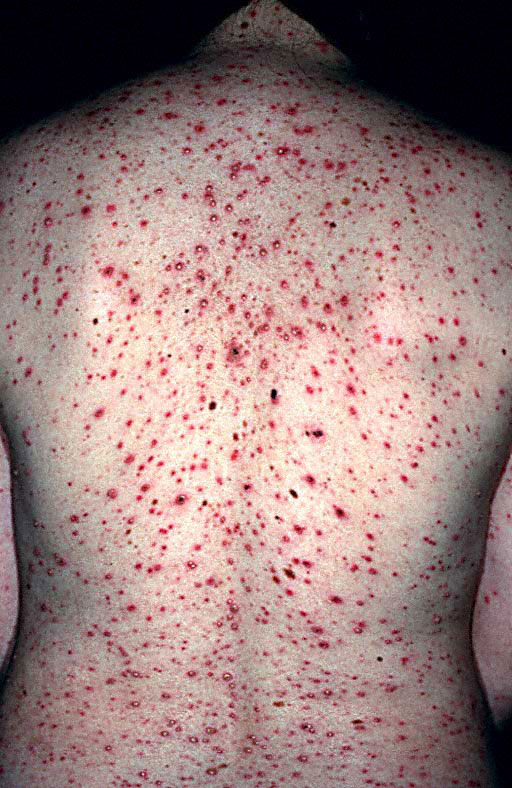
\includegraphics[width=1.2in]{../Imagenes/U.Iowa/Varicela/chicken_pox_picture_01.jpg} &
		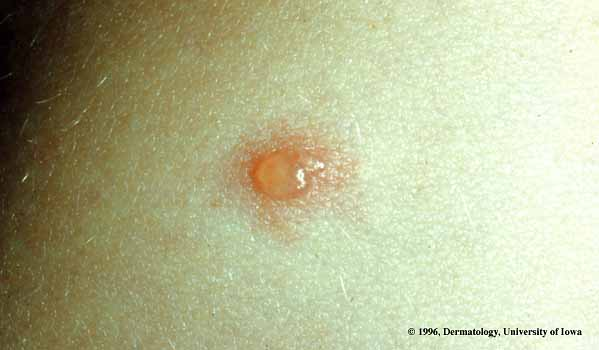
\includegraphics[width=2in]  {../Imagenes/U.Iowa/Varicela/Varicel-02.jpg}
	\end{tabular}
\end{frame}

\begin{frame}
	\frametitle{Elementos que afectan la imagen}
	Problemas
	\begin{itemize}
		\item Ruido \pause
		\item Imperfecciones de la piel \pause
		\item Luces y sombras \pause
		\item Elementos ajenos
	\end{itemize}
\end{frame}

\subsection{T�cnicas utilizadas y medidas adoptadas}
\begin{frame} 
	\frametitle{T�cnicas utilizadas y medidas adoptadas}
	T�cnicas y medidas adoptadas
	\begin{itemize}
		\item Elecci�n de un subconjunto de las im�genes \pause
		\item Ecualizaci�n del histograma (Contrast-limited adaptive histogram equalization) \pause
		\item Reducci�n del ruido o suavizaci�n utilizando un filtro gaussiano \pause
		\item Elecci�n del espacio de color 
	\end{itemize}
\end{frame}

\begin{frame}
	\frametitle{Algunas de las im�genes con las que trabajamos}
	\begin{tabular}{ cc }
		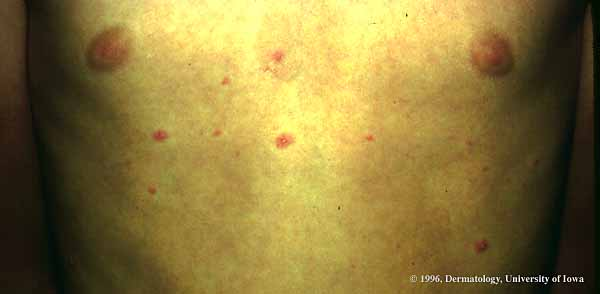
\includegraphics[width=1.6in]{../Imagenes/U.Iowa/Varicela/Varicel-01.jpg} & 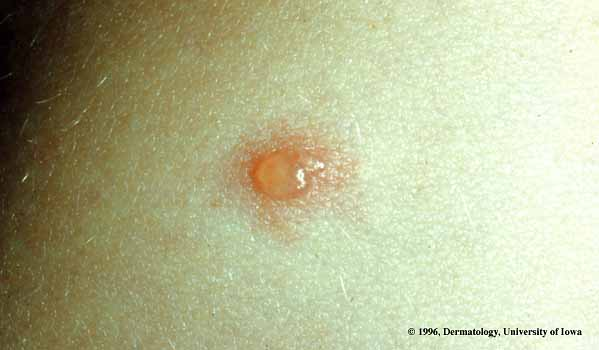
\includegraphics[width=1.6in]{../Imagenes/U.Iowa/Varicela/Varicel-02.jpg} \\
		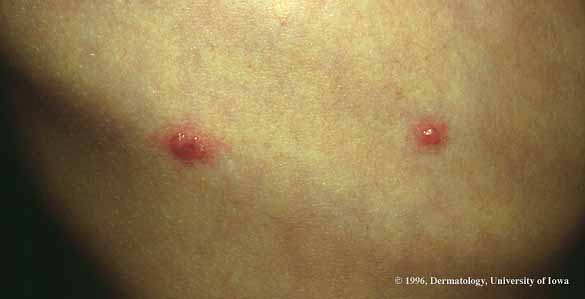
\includegraphics[width=1.6in]{../Imagenes/U.Iowa/Varicela/Varicel-03.jpg} & 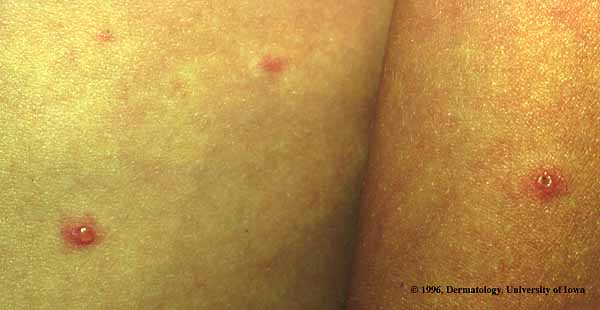
\includegraphics[width=1.6in]{../Imagenes/U.Iowa/Varicela/Varicel-04.jpg} \\
	\end{tabular}
\end{frame}

\begin{frame}
	\frametitle{Algunas de las im�genes con las que trabajamos}
	\begin{tabular}{ cc }
		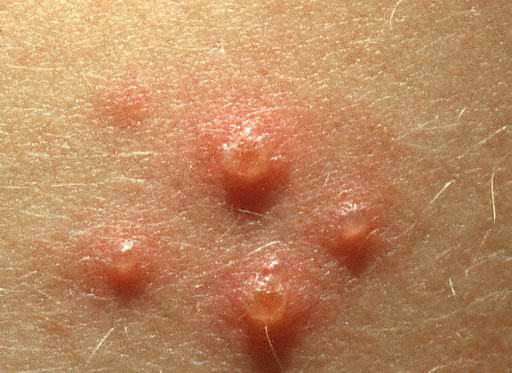
\includegraphics[width=1.6in]{../Imagenes/U.Iowa/Varicela/chicken_pox_primary_lesions_03.jpg} & 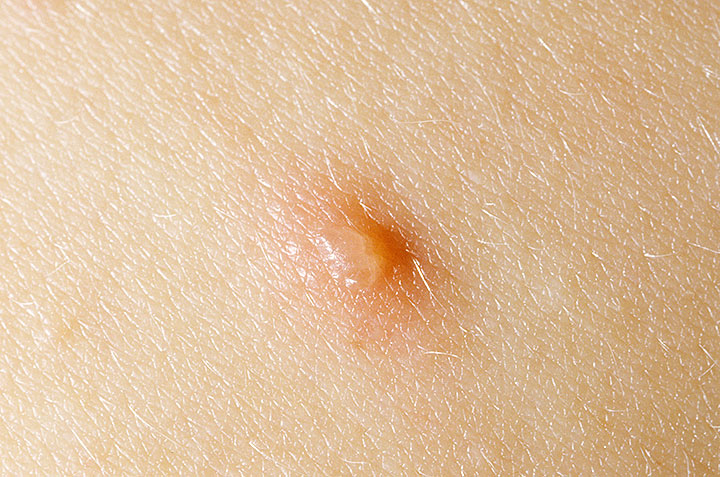
\includegraphics[width=1.6in]{../Imagenes/U.Iowa/Varicela/varicella_20.jpg} \\
	\end{tabular}
\end{frame}